\documentclass{resume} % Use the custom resume.cls style

\usepackage[left=0.75in,top=0.6in,right=0.75in,bottom=0.6in]{geometry} % Document margins
\usepackage{fontawesome}
\usepackage{hyperref}
\hypersetup{
    colorlinks=true,
    linkcolor=blue,
    filecolor=magenta,      
    urlcolor=cyan,
}
\usepackage{graphicx}
% Skill bars filled proportionally
\usepackage{xcolor}
\usepackage{fancyhdr}
\usepackage{array,longtable,picture}
\usepackage{lmodern}
\definecolor{noskillgray}{gray}{0.85}
\definecolor{skilledblue}{rgb}{0.05,0.05,0.65}

\makeatletter
\newdimen\skillb@level
\newdimen\skillb@length
\newdimen\skillb@height
\skillb@length=120pt%
\skillb@height=10pt%
\newcommand*{\skillbar}[1]{%
	\skillb@level=\dimexpr#1\skillb@length/100\relax%
	{\color{skilledblue}\rule{\skillb@level}{\skillb@height}}%
	{\color{noskillgray}%
		\rule{\dimexpr\skillb@length-\skillb@level\relax}{\skillb@height}}%
}
\newcommand*{\skill}[2]{%
	\par\noindent%
	{\hskip 1ex\small #1}\\%
	\skillbar{#2}%
}
\makeatother

% -----------------------------------------------------------------------------
% \noindent % 4cm is the picture's width, -6cm by trial and error

% \begin{picture}(0,0)
% \put(\dimexpr\textwidth-4cm,-6cm){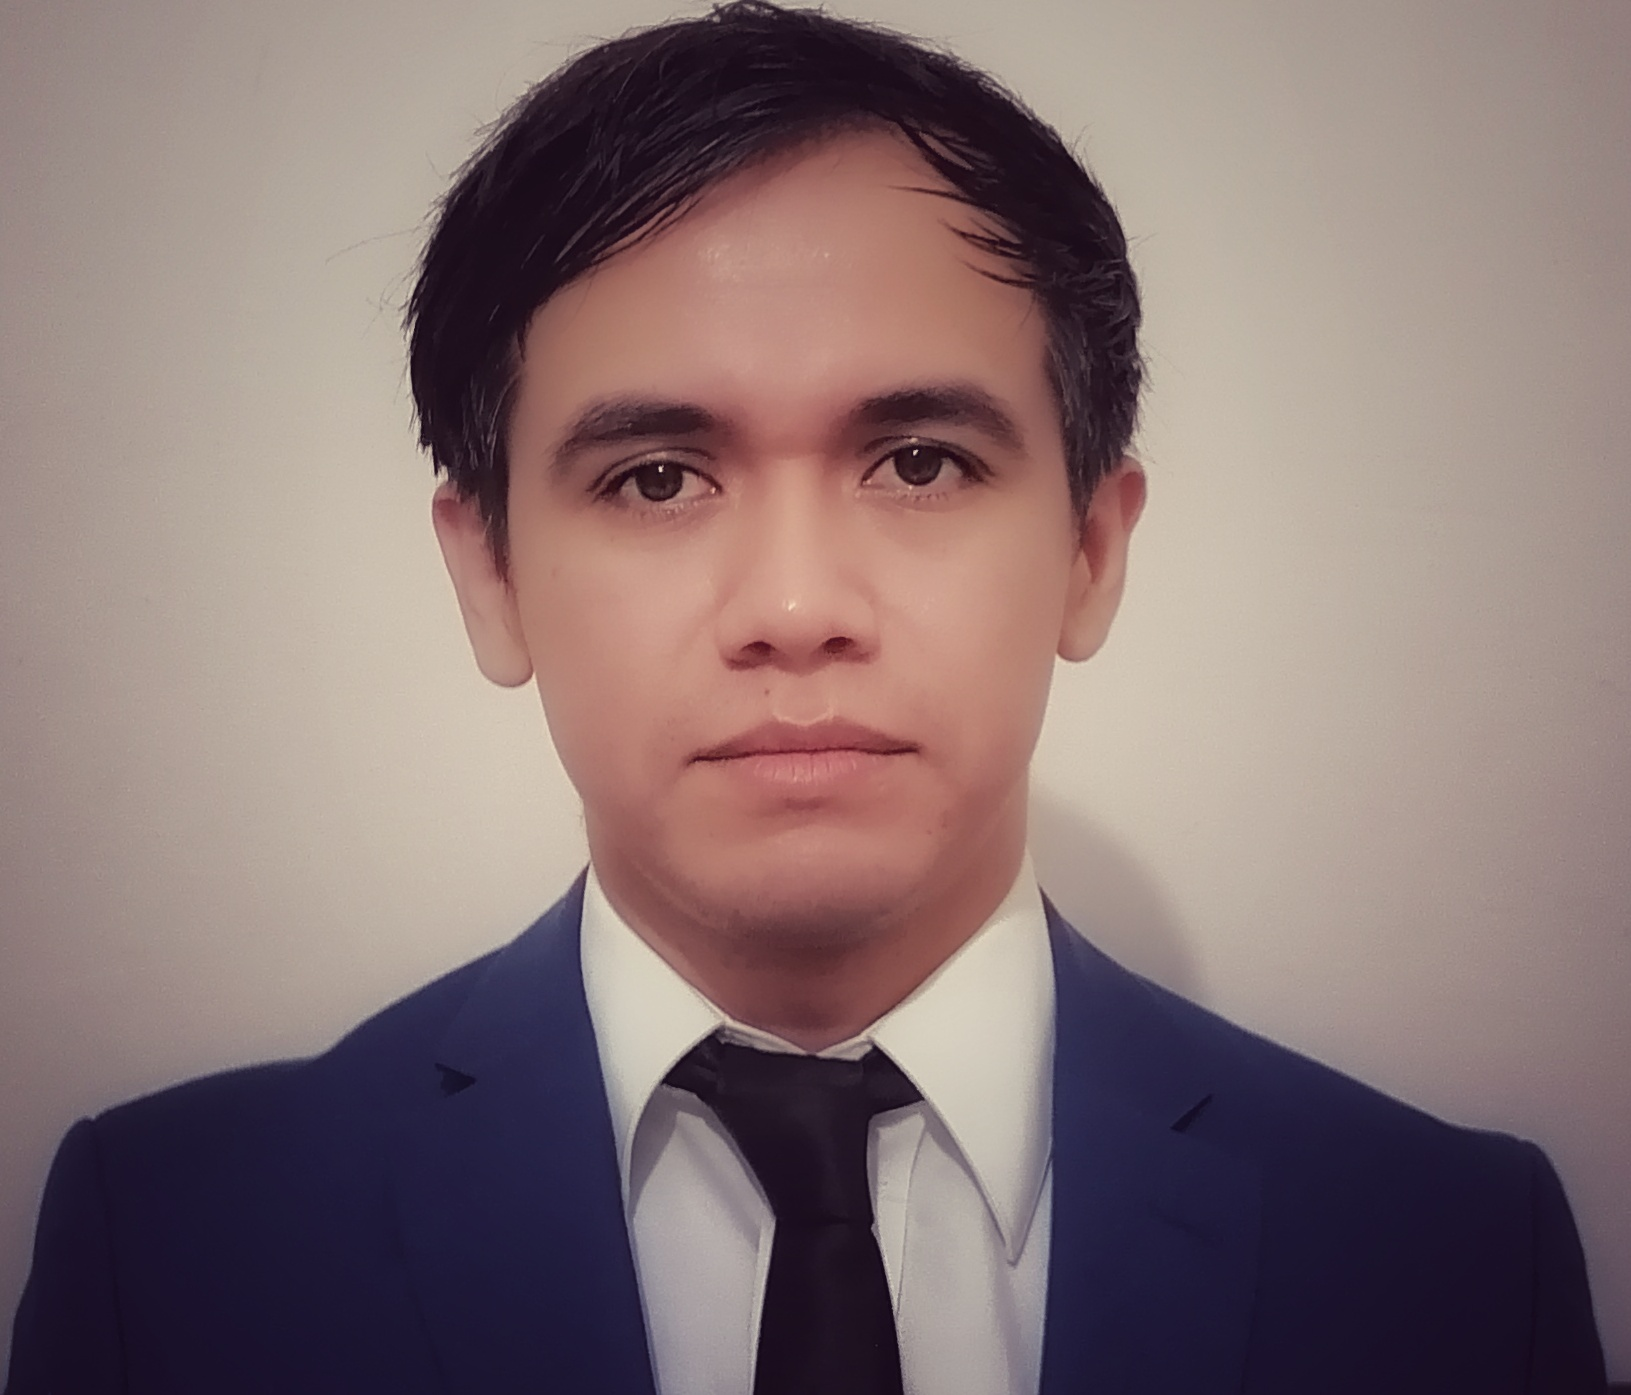
\includegraphics[width=4cm]{pic_CV.jpeg}}
% \end{picture}

\name{Emmanuel Alcalá} % Your name

%\address{123 Broadway \\ City, State 12345} % Your address
%\address{123 Pleasant Lane \\ City, State 12345} % Your secondary addess (optional)
%\address{WebPage: \url{https://jealcalat.github.io/} \tiny{\faExternalLink}} % Your phone number and email
\address{\faMobile \hspace{1ex} {\sf 33 14 99 93 16}}

% \address{e-mail:}
\address{ \faEnvelope \hspace*{0.2em}%
                 \texttt{jealcalat@gmail.com} \\
                 \texttt{jaime.alcala@iteso.mx}}
                 
\address{\faGithub \hspace{1ex} \url{https://github.com/jealcalat}}

\begin{document}
% \thispagestyle{fancy}

% \makecvheader

\begin{picture}(0,0)
    \put(0,-9){\fbox{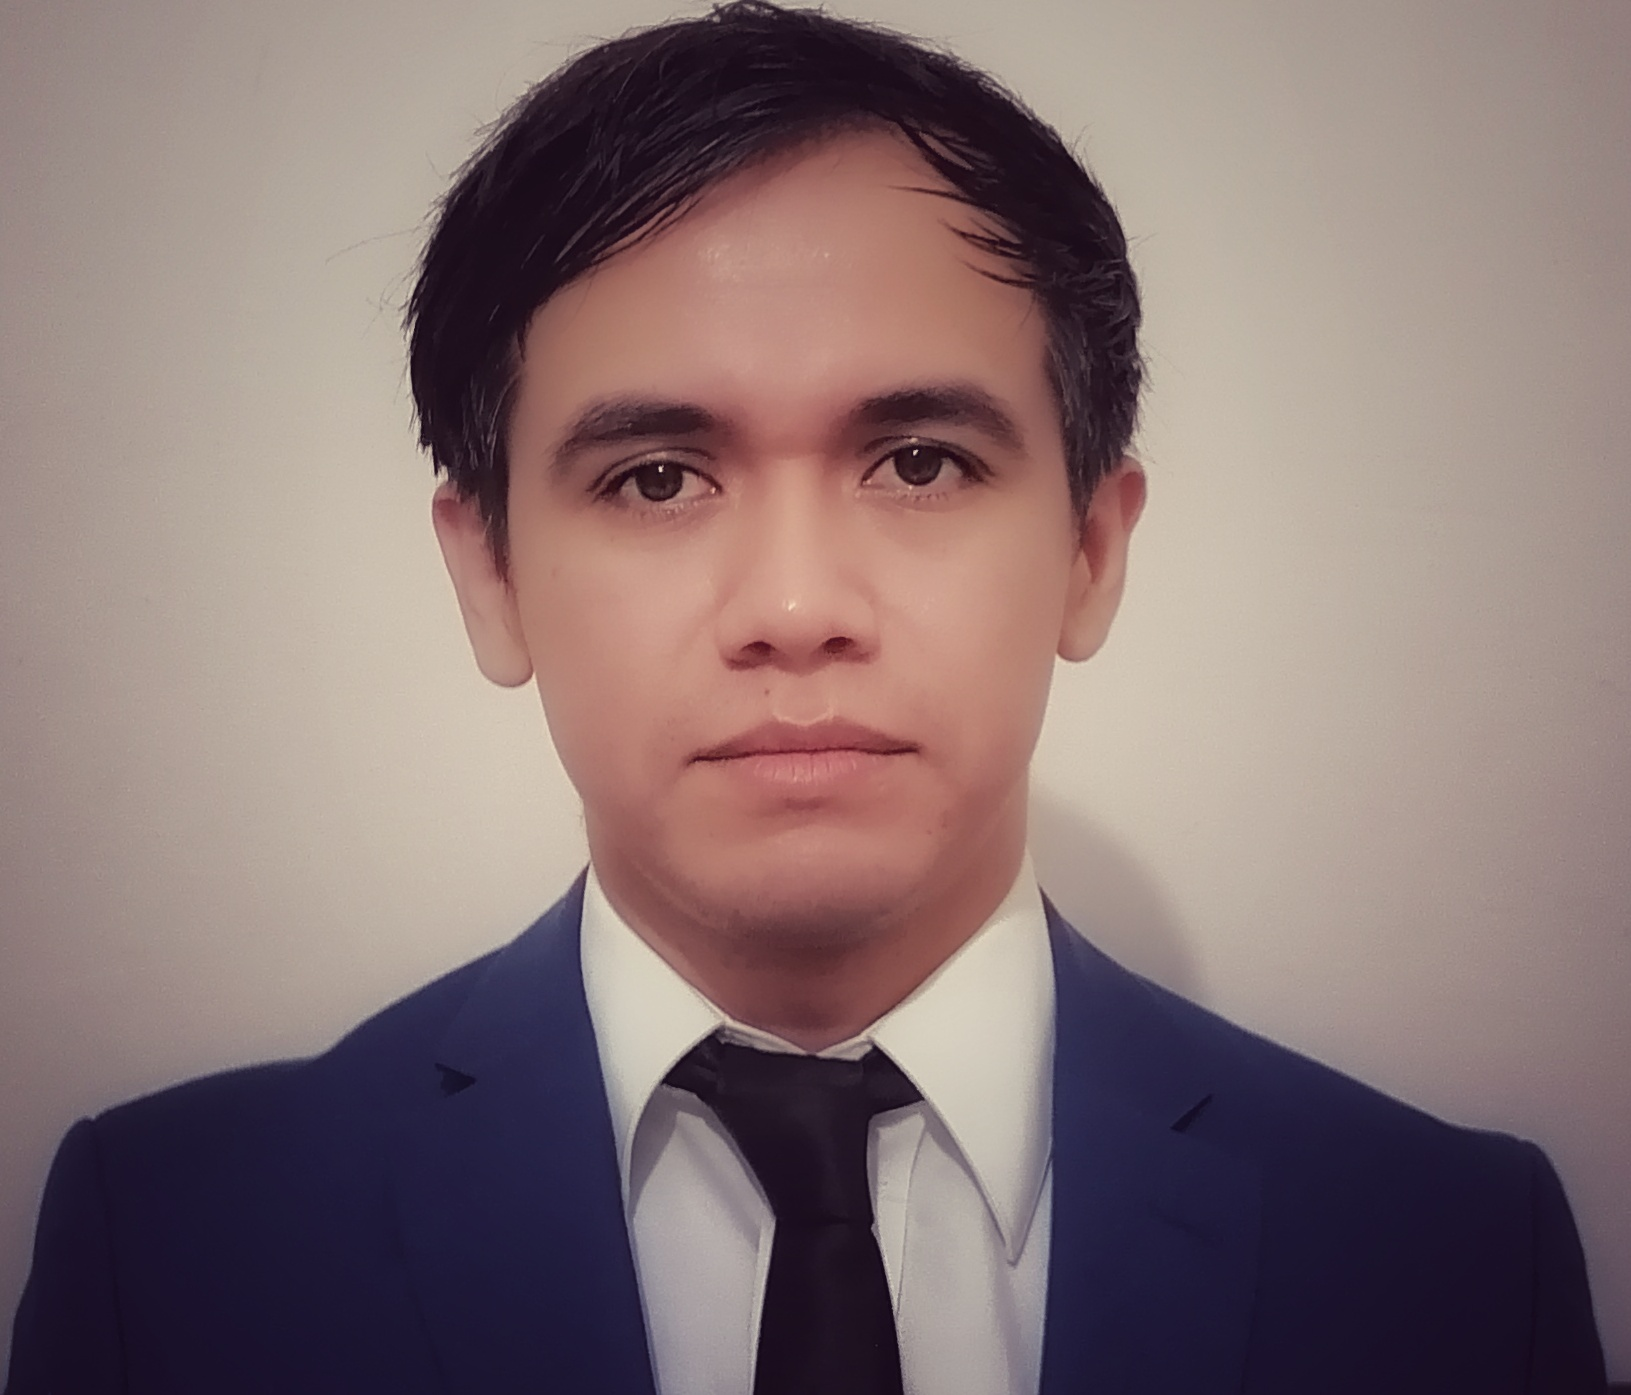
\includegraphics[width=10em]{pic_CV.jpeg}}}
\end{picture}

% \begin{flushright}
% 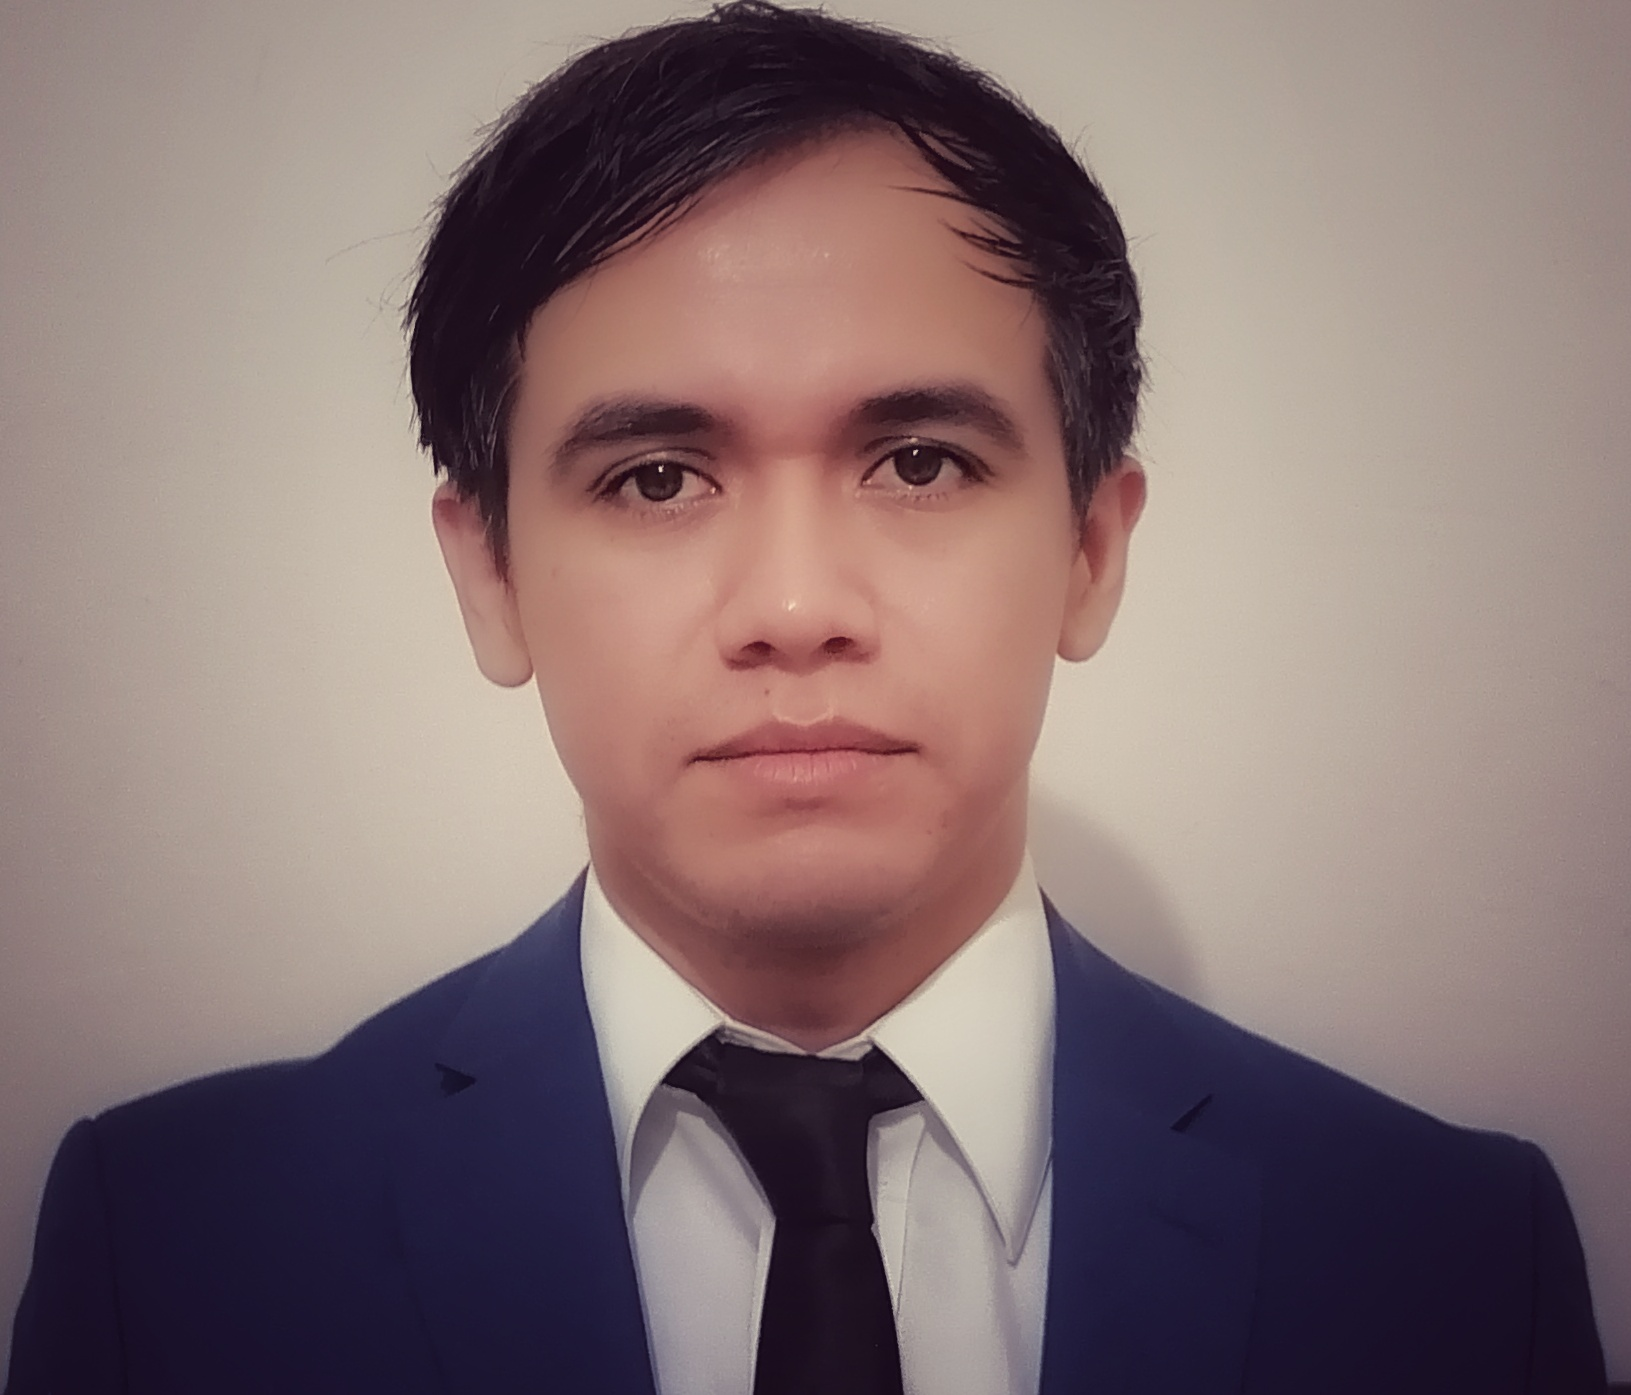
\includegraphics[scale=0.05]{pic_CV.jpeg}
% \end{flushright}

\begin{rSection}{Perfil}
   Tengo una formación ecléctica que me ha facilitado desempeñarme en diversas áreas, tanto educativas como de investigación. En maestría y en doctorado modelé computacionalmente fenómenos de comportamiento económico (toma de decisiones intertemporales y bajo incertidumbre) usando modelos de redes neurales, modelos generativos y probabilísticos. Uno de mis intereses durante ese período fue el uso de IA para estudiar cuantitativamente fenómenos económicos y psicobiológicos, para conocer cómo los seres vivos aprenden estructuras ricas de información imperfecta y bajo incertidumbre. También implementé modelos de visión por computadora, como OpenCV y \textit{posture tracking} (\href{http://www.mackenziemathislab.org/deeplabcut}{DeepLabCut}). Actualmente, me encuentro inmerso en varios proyectos, uno de los cuales requiere del uso Deep Learning para estudiar los trazos y posturas durante la escritura de niños en edad preescolar. En ITESO realicé estancia posdoctoral, y también he impartido las materias de Decisiones y Teoría de Juegos y Econometría. En mi estancia posdoctoral gané experiencia en la implementación de diseños de experimentos, análisis de regresión y en la metodología de superficies de respuesta. Desde el 2022 soy miembro del Sistema Nacional de Investigadores, nivel Candidato.
\end{rSection}

\begin{rSection}{Educación}

{\bf Universidad de Guadalajara, CUCIénega} \hfill {\em 2008 - 2012} \\ 
Lic. Químico Farmacobiólogo \\
% Tesis: OGM y estandarización de Western-Blot \\
{\bf Universidad de Guadalajara, CEIC-CUCBA} \hfill {\em 2015 - 2017} \\ 
Maestría en Ciencias de la Conducta \\
Fecha de examen: 6 de julio de 2017\\
Tesis: Modelo de redes neurales de elección impulsiva \\
{\bf Universidad de Guadalajara, CEIC-CUCBA} \hfill {\em 2017 - 2021} \\
Doctor en Ciencias de la Conducta \\
Fecha de examen: 24 de mayo de 2021\\
Tesis: Formación de hábitos y resistencia al cambio; modelos computacionales

\end{rSection}

\begin{rSection}{Premios y distinciones}

{\bf Miembro de Sistema Nacional de Investigadores - C} \hfill {\em 1 enero 2022 - }\\
Vigencia: 1 enero del 2022 a 31 de diciembre de 2025

\end{rSection}

\begin{rSection}{Publicaciones}

	{\em 2018} \\
	{\bf Alcalá, E.}, \& Arámbula-Román, J.C.(2018). El consumidor contra la democracia, y por qué retomar la psicología no reduccionista. En \textit{Capital social, decentralización y participación ciudadana: entre la reflexión y la evidencia}. (A.R. Cogco-Calderón \& Pérez-Cruz, J.A, Eds). Ciudad de México: UAT-Colofón
	
	{\em 2019} \\
	Buriticá, J.J., \& \textbf{Alcalá, E.} (2019). Increased Generalization in a Peak Procedure after Delayed Reinforcement. \textit{Behavioural Processes, 169, 103978}.
	
	{\em 2020} \\
	Castiello, S., Burgos, J.E., Buriticá, J., dos Santos, C.V. \& \textbf{Alcalá, E.} (2020). Interacción entre magnitud y probabilidad de reforzamiento en la elección automoldeada. \textit{Revista Mexicana de Análisis de la Conducta.}
	
	Gómez, E. G., García, V. I., Morales, C. S., López, F. A. L., \& \textbf{Alcalá, E.} (2020). \textit{Manual de Análisis de Datos de Descuento Temporal en RStudio (MADDTeR)}. Red Universitaria de Aprendizaje (RUA) de la UNAM. \url{https://www.rua.unam.mx/portal/recursos/ficha/85989}
	
	{\em 2021} \\
	
	Eudave-Patiño, M., \textbf{Alcalá, E.,} Valerio dos Santos, C., Buriticá, J., (2021). Similar attention and performance in female and male CD1 mice in the peak procedure. \textit{Behavioural Processes. In Press}. DOI: \url{10.1016/j.beproc.2021.104443}
	
	López-Cárdenas, P.G, \textbf{Alcalá, E.}, Sánchez-Torres, J.D., Araujo, E. (2021). Enhancing the Sensitivity of a Class of Sensors: A Data-Based Engineering Approach. \textit{2021 IEEE 21st International Conference on Nanotechnology (NANO)}, 221-224, DOI: \url{10.1109/NANO51122.2021.9514352}. 
	
	López-Cárdenas, P. G.,\textbf{ Alcalá, E.}, Sánchez-Torres, J. D., \& Araujo, E. (2021, November). A Resampling Approach for the Data-Based Optimization of Nanosensors. In \textit{2021 18th International Conference on Electrical Engineering, Computing Science and Automatic Control (CCE) (pp. 1-4). IEEE.}
	
	{\em 2022}\\ 
	
	Campos-Ordoñez, T.,\textbf{Alcalá, E.}, Ibarra-Castañeda, N., Buriticá, J., González-Pérez, 0. (2021). A repeated cyclohexane inhalation generates stereotypic circling, hyperlocomotion, persistent anxiety-like behavior, and dysregulates the c-Fos expression in striatum and nucleus accumbens. \textit{Behavioural brain research, 418, 113664}
	
	Sosa, R., \textbf{Alcalá., E}. (2022). The Nervous System as a Solution for Implementing Closed Negative Feedback Control Loops. \textit{Journal of Experimental Analysis of Behavior}, 1-22

	{\em 2023}\\

	López-Cárdenas, P. G.,\textbf{ Alcalá, E.}, Sánchez-Torres, J. D., \& Araujo, E. (2023). Improving self-supported nanowire arrays using response surface methodology for the synthesis of a H2O2 nanostructured sensor. \textit{Materials Chemistry and Physics, 303, 127729}
	
	\textbf{Alcalá, E.}, Márquez, I., Lara, E., Cabrera, F. \& Buriticá, J. (2023). Asignación de tiempo para responder o no-responder en un procedimiento de degradación de contingencia. \textit{Revista Mexicana de Análisis de la Conducta.49-1, 65-87.}	

	\end{rSection}

\begin{rSection}{Experiencia}

\begin{rSubsection}{CEIC, Universidad de Guadalajara}{2022-2024}{Investigador Posdoctoral}{CONAHCyT}
	\item Caracterización computacional y conductual de la exposición a inhalables en modelos murinos.
\end{rSubsection}

\begin{rSubsection}{ITESO}{2021}{Posdoctorado}{COECYTJAL - Proyecto FODECYJAL 8248-2019}
\item Diseños experimentales, análisis de datos y optimización mediante superficies de respuesta.
\end{rSubsection}

\begin{rSubsection}{ITESO}{2021}{Profesor}{}
    \item Decisiones y Teoría de Juegos en Ingeniería Financiera.
    \item Econometría Básica en la Licenciatura de Gestión Pública y Políticas Globales.
\end{rSubsection}

\begin{rSubsection}{Universidad de la Ciénega}{2019}{Profesor}{Guadalajara, Jal}
\item Clases de bioestadística para la carrera de Nutrición
\end{rSubsection}

\begin{rSubsection}{Consultor ({\em freelancer})}{2018 - }{Análisis de datos y asesoría estadística}{Guadalajara, Jal}
\item Diseño experimental, análisis de datos e inferencia estadística para la toma de decisiones
\item Ejemplo de trabajo: Hospital San Javier, Fistula Day:  \url{https://bit.ly/2Vz2sl7}
\end{rSubsection}

\begin{rSubsection}{UTEG}{2017}{Asesor académico}{Guadalajara, Jal.}
	\item Asesor y tutor de estudiantes talento.
\end{rSubsection}

%------------------------------------------------

\begin{rSubsection}{Instituto Lumiere}{2014 - 2015}{Instructor}{Ocotlán, Jal}
	\item Resolución de problemas de álgebra y cálculo
\end{rSubsection}

\end{rSection}

% Publications


\begin{rSection}{Ponencias y carteles}
{\em 2016} \hfill {\em CUCosta, UdeG, Jalisco} \\
{\bf XXVI Congreso Mexicano de Análisis de la conducta} (Ponencia) \\
Elección automoldeada en redes neurales: sensibilidad a la magnitud y probabilidad de reforzamiento. 

{\em 2017} \hfill {\em UAA, Aguascalientes} \\
{\bf XXVII Congreso Mexicano de Análisis de la conducta} (Ponencia) \\
Impulsividad pavloviana: predicción y prueba de un modelo de redes neurales artificiales. 

{\bf XXVII Congreso Mexicano de Análisis de la conducta} (Ponencia) \\ 
Modelo de redes neurales DDS: herramientas teóricas, predicciones experimentales y una implementación robótica.

{\em 2019} \hfill {\em UNAM-INB, Querétaro} \\
{\bf 2nd Annual Conference of the Timing Research Forum} (Cartel) \\
Increased Generalization after Delayed Reinforcement

{\bf Seminario Internacional sobre Comportamiento y Aplicaciones (SINCA) VIII } (Cartel)
Aplicaciones de aprendizaje estadıstico a estimación temporal con programas de intervalo fijo.\\
\href{https://www.researchgate.net/profile/Emmanuel-Alcala/publication/352672052_Aplicaciones_de_aprendizaje_estadistico_a_estimacion_temporal_con_programas_de_intervalo_fijo/links/60d29f2592851c34e07cdd31/Aplicaciones-de-aprendizaje-estadistico-a-estimacion-temporal-con-programas-de-intervalo-fijo.pdf}{SINCA VIII 2019}

\end{rSection}

\begin{rSection}{Habilidades técnicas {\normalfont (0 - 100 \%)}}

%\begin{tabular}{ @{} >{\bfseries}l @{\hspace{6ex}} l }
%Computer Languages & Prolog, Haskell, AWK, Erlang, Scheme, ML \\
%Protocols \& APIs & XML, JSON, SOAP, REST \\
%Databases & MySQL, PostgreSQL, Microsoft SQL \\
%Tools & SVN, Vim, Emacs
%\end{tabular}

\begin{tabular} { @{} >{\bf}l @{\hspace{6ex}} l }
	\skill{\sf R \& RStudio (IDE)}{70} & Lenguaje, software estadístico y múltiples librerías \\
	\skill{\sf Python 3}{45} & Lenguaje, OpenCV y scikit-learn\\
	\skill{\LaTeXe}{65} & Preparación de documentos científicos técnicos\\
	\skill{Sistemas Operativos}{70} & Windows, Linux (shell scripting básico) y macOS
\end{tabular}

\end{rSection}

\begin{rSection}{Formación adicional}
	{\em 2016}  \\
	{\bf Teoría de la probabilidad y estadística matemática} \hfill {\em CUCEI, UdG}
	
	{\bf Data Science Bootcamp} \hfill {\em IBM-UdG}

	{\em 2017} \\
	{\bf Model comparison in quantitative analysis of behavior} \hfill {UAA - Randolph Grace, PhD} 
	
	{\bf Curso de Álgebra lineal} \hfill {\em CUCEI, UdG}
	
\end{rSection}

% \begin{rSection}{Acerca de mí}
% Tengo interés en psicología experimental, ciencias cognitivas, neurociencias, estadística y modelación matemática de fenómenos sociales y cognitivos. Por ejemplo, \href{https://gershmanlab.com/index.html}{CCNlab}, o \href{https://nivlab.princeton.edu/}{Niv Lab}, cuya investigación es mi aspiración personal. Después de obtener el grado, decidí estudiar posgrado en Análisis de la Conducta en el Centro de Estudios e Investigaciones en Comportamiento (CEIC), único centro especializado en esos temas en México. Actualmente investigo mecanismos de aprendizaje y modelos de persistencia. Abogo por el software libre, el uso de Linux, Ciencia Abierta y conocimiento libre y reproducibilidad en la ciencia. Tengo un fuerte interés por la filosofía y, fuera de lo académico, por la literatura y cine. 
% \end{rSection}


\end{document}
